\documentclass{beamer}

%%%%%%%%%%%%%Solarized Theme%%%%%%%%%%%%%%%
\usecolortheme[dark,accent=cyan]{solarized}
\beamertemplatenavigationsymbolsempty
%%%%%Packages%%%%%
\usefonttheme{serif}
\usepackage[T1]{fontenc}
\usepackage[utf8]{inputenc}
\usepackage[english]{babel}
\usepackage{fontawesome}
\usepackage{minted}

\definecolor{DarkGray}{gray}{0.1}
\usemintedstyle{paraiso-dark}


\usepackage{graphicx}
\usepackage{hyperref}
\usepackage{colortbl, xcolor}
\usepackage{booktabs}
\usepackage{amsmath,amsthm, amssymb, latexsym}

\usepackage{tikz}
\usepackage{standalone}
\usepackage{siunitx}
\usetikzlibrary{calc, positioning, arrows, arrows.meta, shapes, automata}
\usetikzlibrary{backgrounds, fit}
\makeatletter
\newcommand{\srcsize}{\@setfontsize{\srcsize}{5pt}{5pt}}
\makeatother
\usepackage{tikz}
\usetikzlibrary{er,positioning, calc, patterns, arrows, calc, positioning, arrows, arrows.meta, shapes, automata}
\usetikzlibrary{decorations.pathreplacing, backgrounds, fit}
\tikzset{
    ultra thick/.style={line width=1.6pt},
    % Define standard arrow tip
    >=stealth',
    % Define style for boxes
    chain/.style={
        rectangle, 
        rounded corners, 
        % fill=black!10,
        draw=white, very thick,
        text width=3.5em, 
        minimum height=3em, 
        text centered},
    punkt/.style={
           ellipse,
           draw=orange,
           ultra thick,
           text width=18em,
           minimum height=8em,
           text centered,
           font=\LARGE},
    % Define arrow style
    pil/.style={
           ->,
           ultra thick,
           draw=orange,
           shorten <=2pt,
           shorten >=2pt,},
    doublepil/.style={
     latex'-latex',
     ultra thick,
     draw=orange,
     shorten <=2pt,
     shorten >=2pt,},
     emojis/.style={
        ellipse,
        text width=17em,
        minimum height=8em,
        text centered,
        font=\LARGE},
}

\begin{document}

\begin{frame}
    \begin{center}
        \large{\textbf{\textcolor{orange}{Understanding responses to environments for the Prisoner's Dilemma:
		A meta analysis, multidimensional optimisation and machine learning approach}}} \\

        \vspace{1cm}
        \normalsize{Nikoleta E. Glynatsi}

        \vspace{1cm}
        \footnotesize{Dr Vincent Knight \& Dr Jonathan Gillard}

    \end{center}
\end{frame}

\begin{frame}
    \begin{center}
    \begin{minipage}{.45\textwidth}
        
\includegraphics[width=0.45\textwidth]{static/ukie.png}
        
\includegraphics[width=0.45\textwidth]{static/stem.jpg} \vspace{.5cm} \\
        \centering
        International Conference \\ on Social Dilemmas
    \end{minipage} \hfill \pause
    \begin{minipage}{.45\textwidth}
        
\includegraphics[width=0.45\textwidth]{static/green_snake.png}
        
\includegraphics[width=0.45\textwidth]{static/logo2020.png} \vspace{.3cm} \\
        
\includegraphics[width=0.45\textwidth]{static/balkan.jpg}
        
\includegraphics[width=0.45\textwidth]{static/euroscipy_logo.png}
    \end{minipage} \vfill
\end{center}
\end{frame}

\begin{frame}
    \begin{center}
    Software Sustainability Institute - Collaborations Workshop \vspace{.5cm} \\
    SoapBox Science Cardiff \vspace{.5cm} \\
    Enriching Student Life Award \vspace{.5cm} \\
    SIAM-IMA Chapter Treasurer \& President
    \end{center}
\end{frame}

\begin{frame}
    \footnotesize{\textcolor{orange}{Published}}
    \tiny{
    \begin{enumerate}
    \def\labelenumi{\arabic{enumi}.}
    \item
    Reinforcement learning produces dominant strategies for
    the Iterated Prisoner's Dilemma. Marc Harper, Vincent Knight, Martin
    Jones, Georgios Koutsovoulos, \textbf{Nikoleta E. Glynatsi}, Owen Campbell -
    \href{https://journals.plos.org/plosone/article?id=10.1371/journal.pone.0188046}{PLOS
    One} -
    \href{https://arxiv.org/abs/1707.06307}{Preprint arXiv:1707.06307}
    \item
    An evolutionary game theoretic model of rhino horn
    devaluation. \textbf{Nikoleta E. Glynatsi}, Vincent Knight, Tamsin Lee.
    \href{https://www.sciencedirect.com/science/article/pii/S0304380018303260}{Ecological
    Modelling} -
    \href{https://arxiv.org/abs/1712.07640}{Preprint arXiv:1712.07640}
    \item
    Evolution reinforces cooperation with the emergence of
    self-recognition mechanisms: an empirical study of the Moran process
    for the Iterated Prisoner's dilemma. Vincent Knight, Marc Harper,
    \textbf{Nikoleta E. Glynatsi}, Owen Campbell -
    \href{https://journals.plos.org/plosone/article/comments?id=10.1371/journal.pone.0204981}{PLOS
    ONE} -
    \href{https://arxiv.org/abs/1707.06920}{Preprint arXiv:1707.06920}
    \item
    An open framework for the reproducible study of the
    Iterated prisoner's dilemma. Vincent Knight, Owen Campbell, Marc
    Harper et al -
    \href{https://openresearchsoftware.metajnl.com/articles/10.5334/jors.125/}{Journal
    of Open Research Software}
    \end{enumerate}
    }
    
    \footnotesize{\textcolor{orange}{Under review}}
    \tiny{
    \begin{enumerate} \def\labelenumi{\arabic{enumi}.}
        \item A bibliometric study of research topics, collaboration and influence in the field of the Iterated Prisoner's Dilemma.
        \textbf{Nikoleta E. Glynatsi} and Vincent A. Knight -
        Palgrave Communications - \href{https://arxiv.org/abs/1911.12112}{Preprint arXiv:1911.06128}
        \item Game Theory and Python: An educational tutorial to game
        theory and repeated games using Python \textbf{Nikoleta E. Glynatsi} and Vincent A. Knight -
        Journal of Open Source Education
        \href{https://github.com/Nikoleta-v3/Game-Theory-and-Python}{Nikoleta-v3/Game-Theory-and-Python}
        \item A theory of mind: Best responses to memory-one strategies.
        The limitations of extortion and restricted memory. \textbf{Nikoleta E. Glynatsi} and Vincent A. Knight -
        Scientific Reports -
        \href{https://arxiv.org/abs/1911.12112}{Preprint arXiv:1911.12112}
    \end{enumerate}
    }
    
    \footnotesize{\textcolor{orange}{In preparation}}
    \tiny{
    \begin{enumerate} \def\labelenumi{\arabic{enumi}.}
    \item Properties of Winning Iterated Prisoner's Dilemma Strategies. \textbf{Nikoleta E. Glynatsi}, Vincent A. Knight
    and Marc Harper
    - \href{https://arxiv.org/abs/2001.05911}{Preprint arXiv:2001.05911}
    \item Recognising and evaluating the effectiveness of extortion in
    the Iterated Prisoner's Dilemma. Vincent Knight, Marc Harper, \textbf{Nikoleta E. Glynatsi},
    Jonathan Gillard -
    \href{https://arxiv.org/abs/1904.00973}{Preprint arXiv:1904.00973}
    \end{enumerate}
    }
    \end{frame}

\begin{frame}
    \begin{center}
    \includestandalone[width=\textwidth]{static/structure}
    \end{center}
\end{frame}

\begin{frame}
    \begin{center}
        \large{``A bibliometric study of research topics, collaboration and influence in the field of the Iterated Prisoner's Dilemma''} \\ \vspace{.5cm}
        \footnotesize{Nikoleta E. Glynatsi, Vincent A. Knight} \\ \vspace{.5cm}
        \footnotesize{arxiv.org/abs/1911.06128} \\ \vspace{.5cm}
        \footnotesize{Under review: Palgrave Communications}
    \end{center}
\end{frame}

\begin{frame}
    \begin{center}
    \includestandalone[width=\textwidth]{static/topics}
    \end{center}
\end{frame}

\begin{frame}
    \begin{center}
        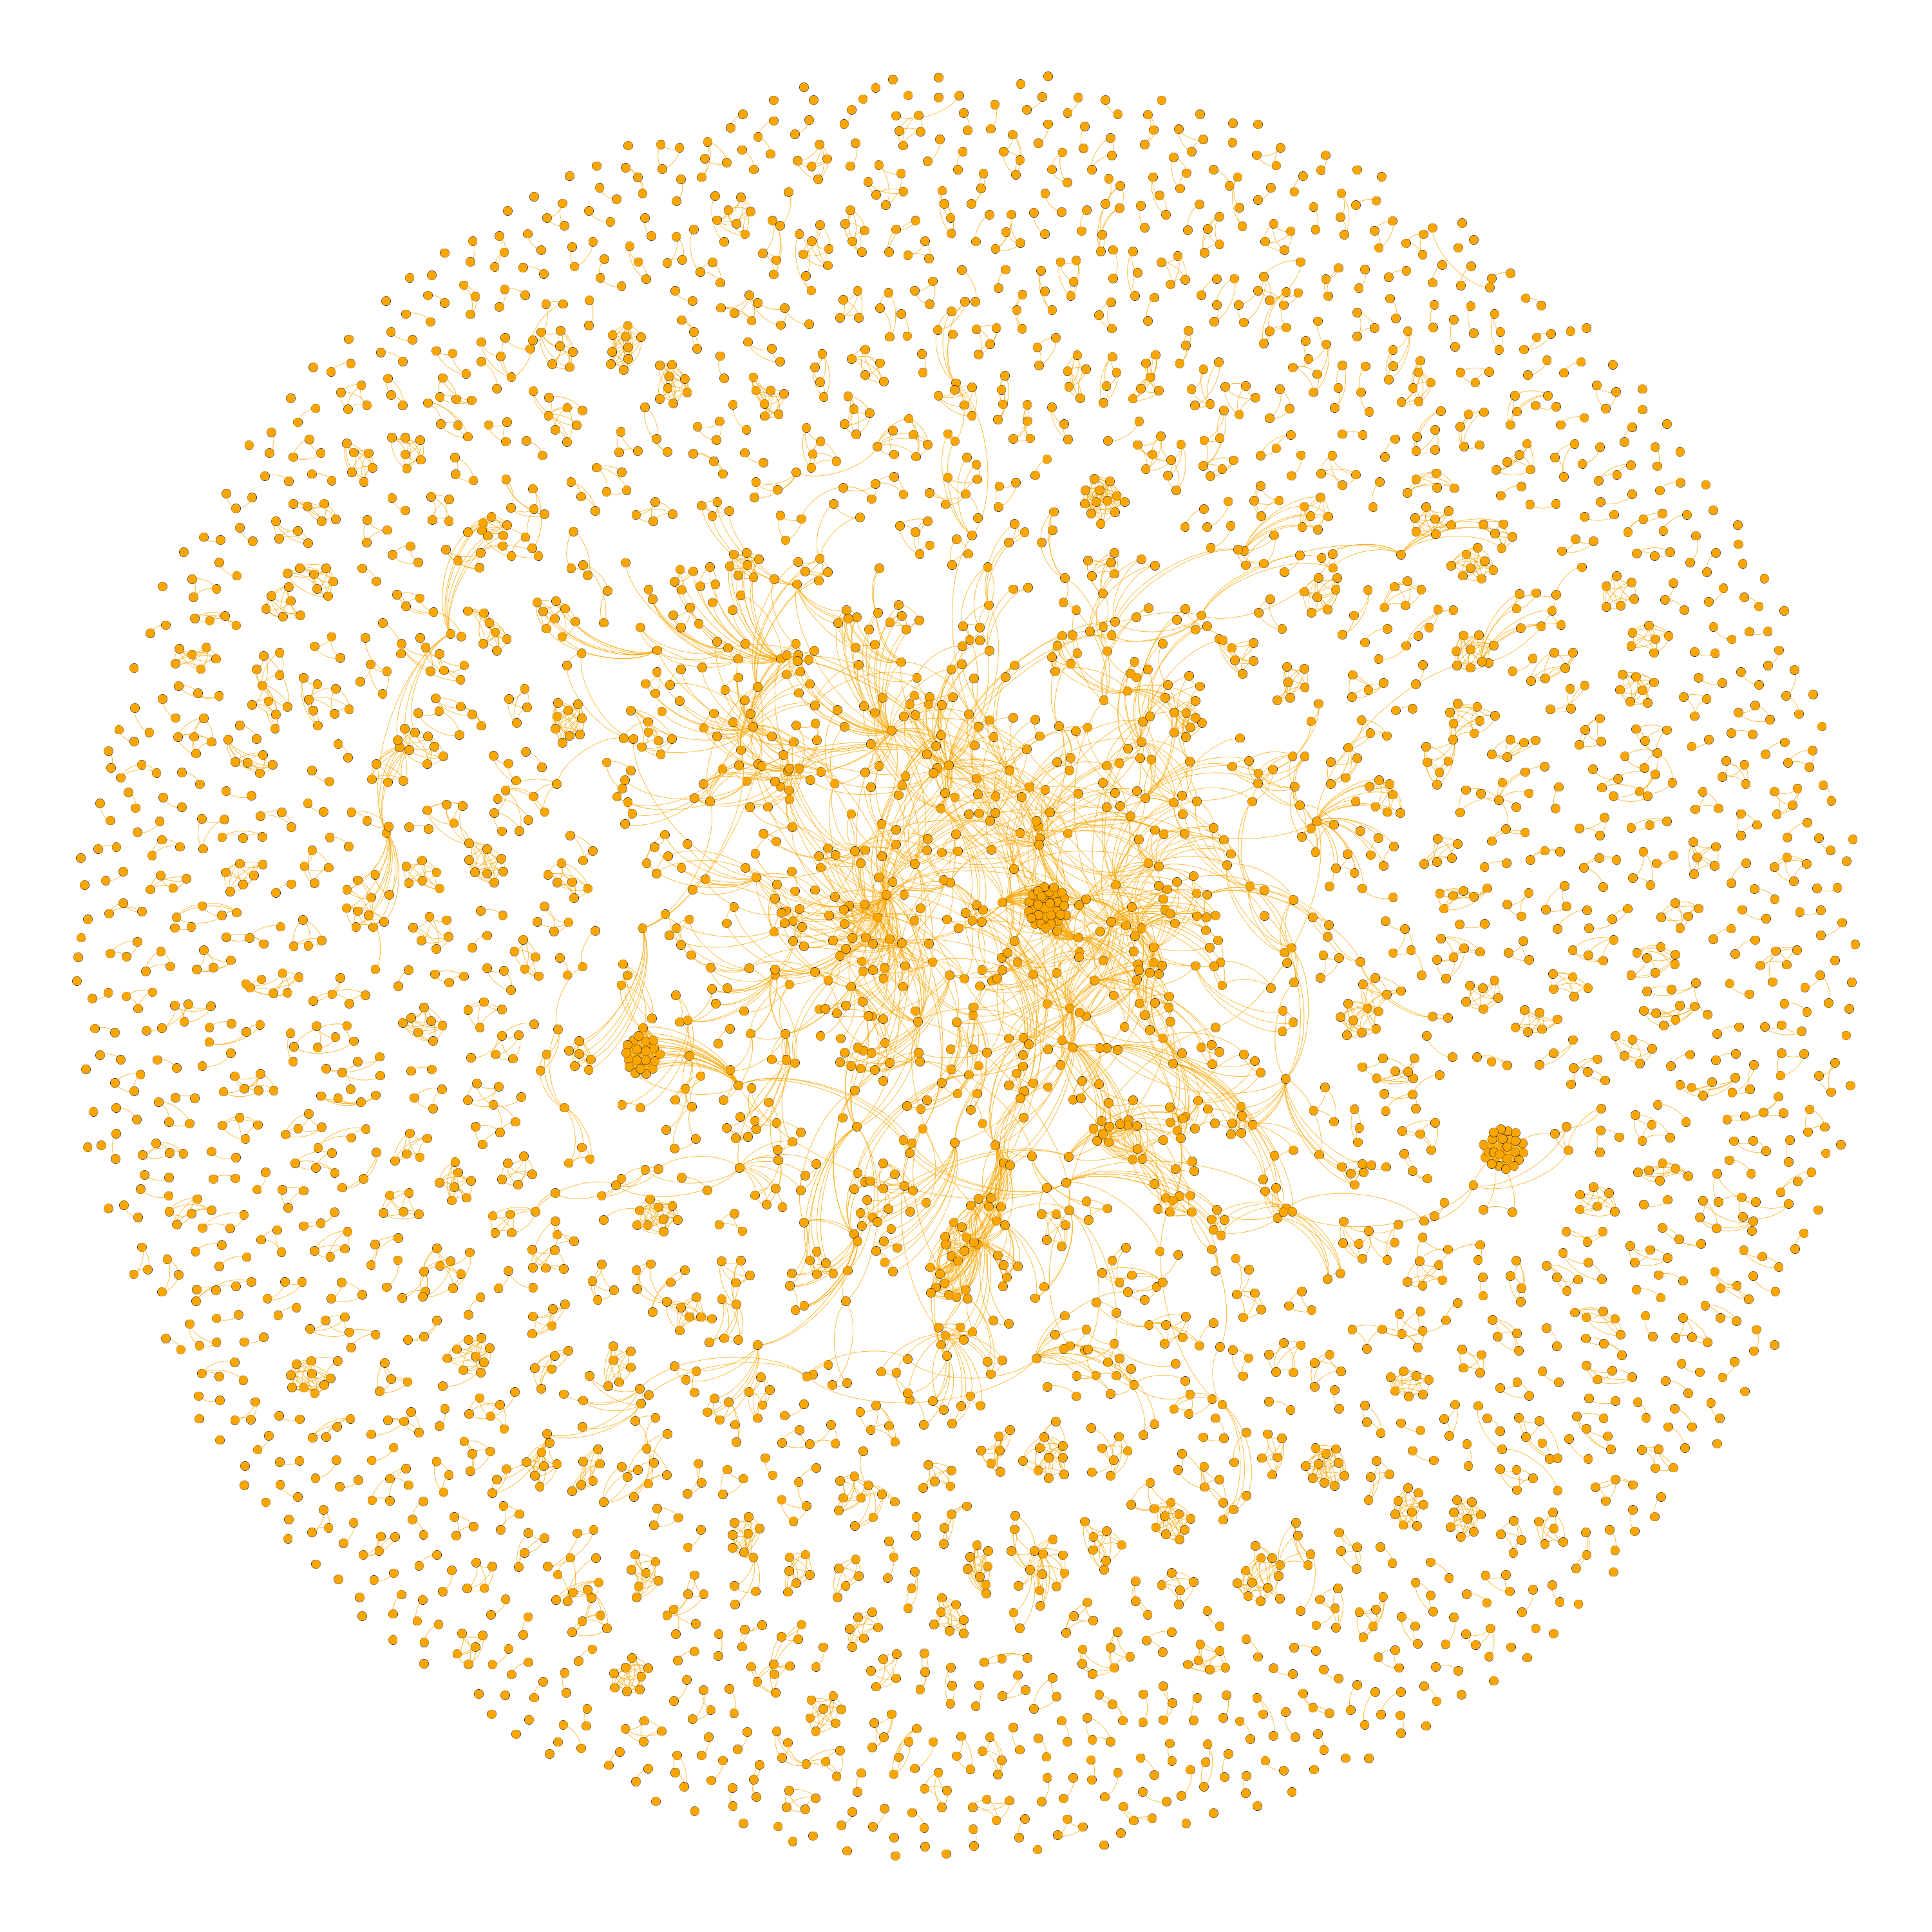
\includegraphics[width=.7\textwidth]{static/pd.png}
    \end{center}
\end{frame}

\begin{frame}
    \begin{center}
        \Large{\textbf{\textcolor{orange}{Highlights \& Challenges}}}
    \end{center}
    \vspace{.8cm} \pause

    \begin{minipage}{.5\textwidth}
        \(\bullet\) ARCAS  \vspace{.1cm} \\ \pause
        \(\bullet\) Large data set \vspace{.1cm} \\ \pause
        \(\bullet\) Natural Language Processing  \vspace{.1cm} \\ \pause
        \(\bullet\) Concrete insights from textual data \pause
    \end{minipage} \hfill
    \begin{minipage}{.45\textwidth}
        \(\bullet\) Understanding journals protocols \vspace{.1cm} \\ \pause
        \(\bullet\) Cleaning data \\
    \end{minipage}
\end{frame}

\begin{frame}
    \begin{center}
        \large{``Properties of Winning Iterated Prisoner's Dilemma Strategies''} \\ \vspace{.5cm}
        \footnotesize{Nikoleta E. Glynatsi, Vincent A. Knight, Marc Harper} \\ \vspace{.5cm}
        \footnotesize{arXiv:2001.05911} \\ \vspace{.5cm}
        \footnotesize{data: DOI:10.5281/zenodo.3516652}
    \end{center}
\end{frame}

\begin{frame}
    \begin{center}
        \textbf{Tit For Tat Normalised Rank} \\ \vspace{1cm}
        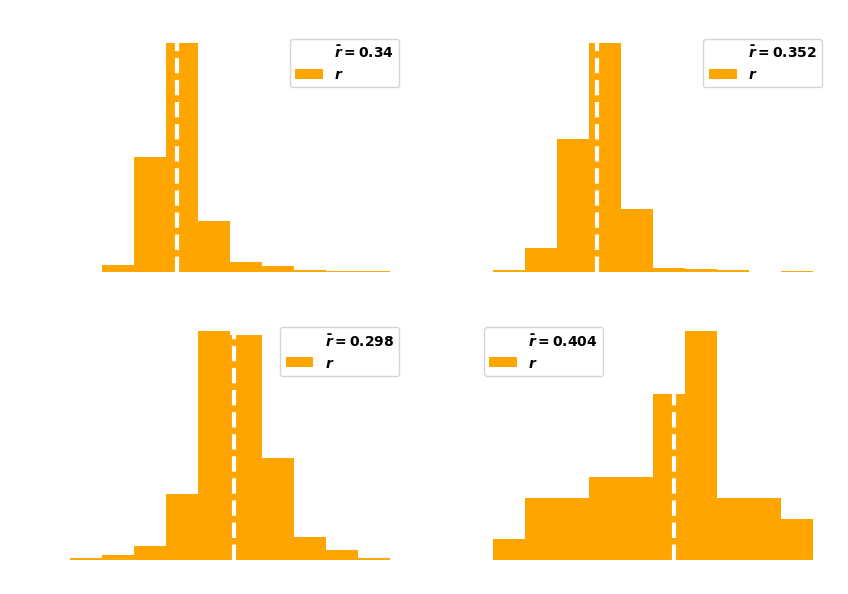
\includegraphics[width=.8\textwidth]{static/tit_for_tat_r_distributions.png} 
    \end{center}
\end{frame}

\begin{frame}
    \begin{center}
        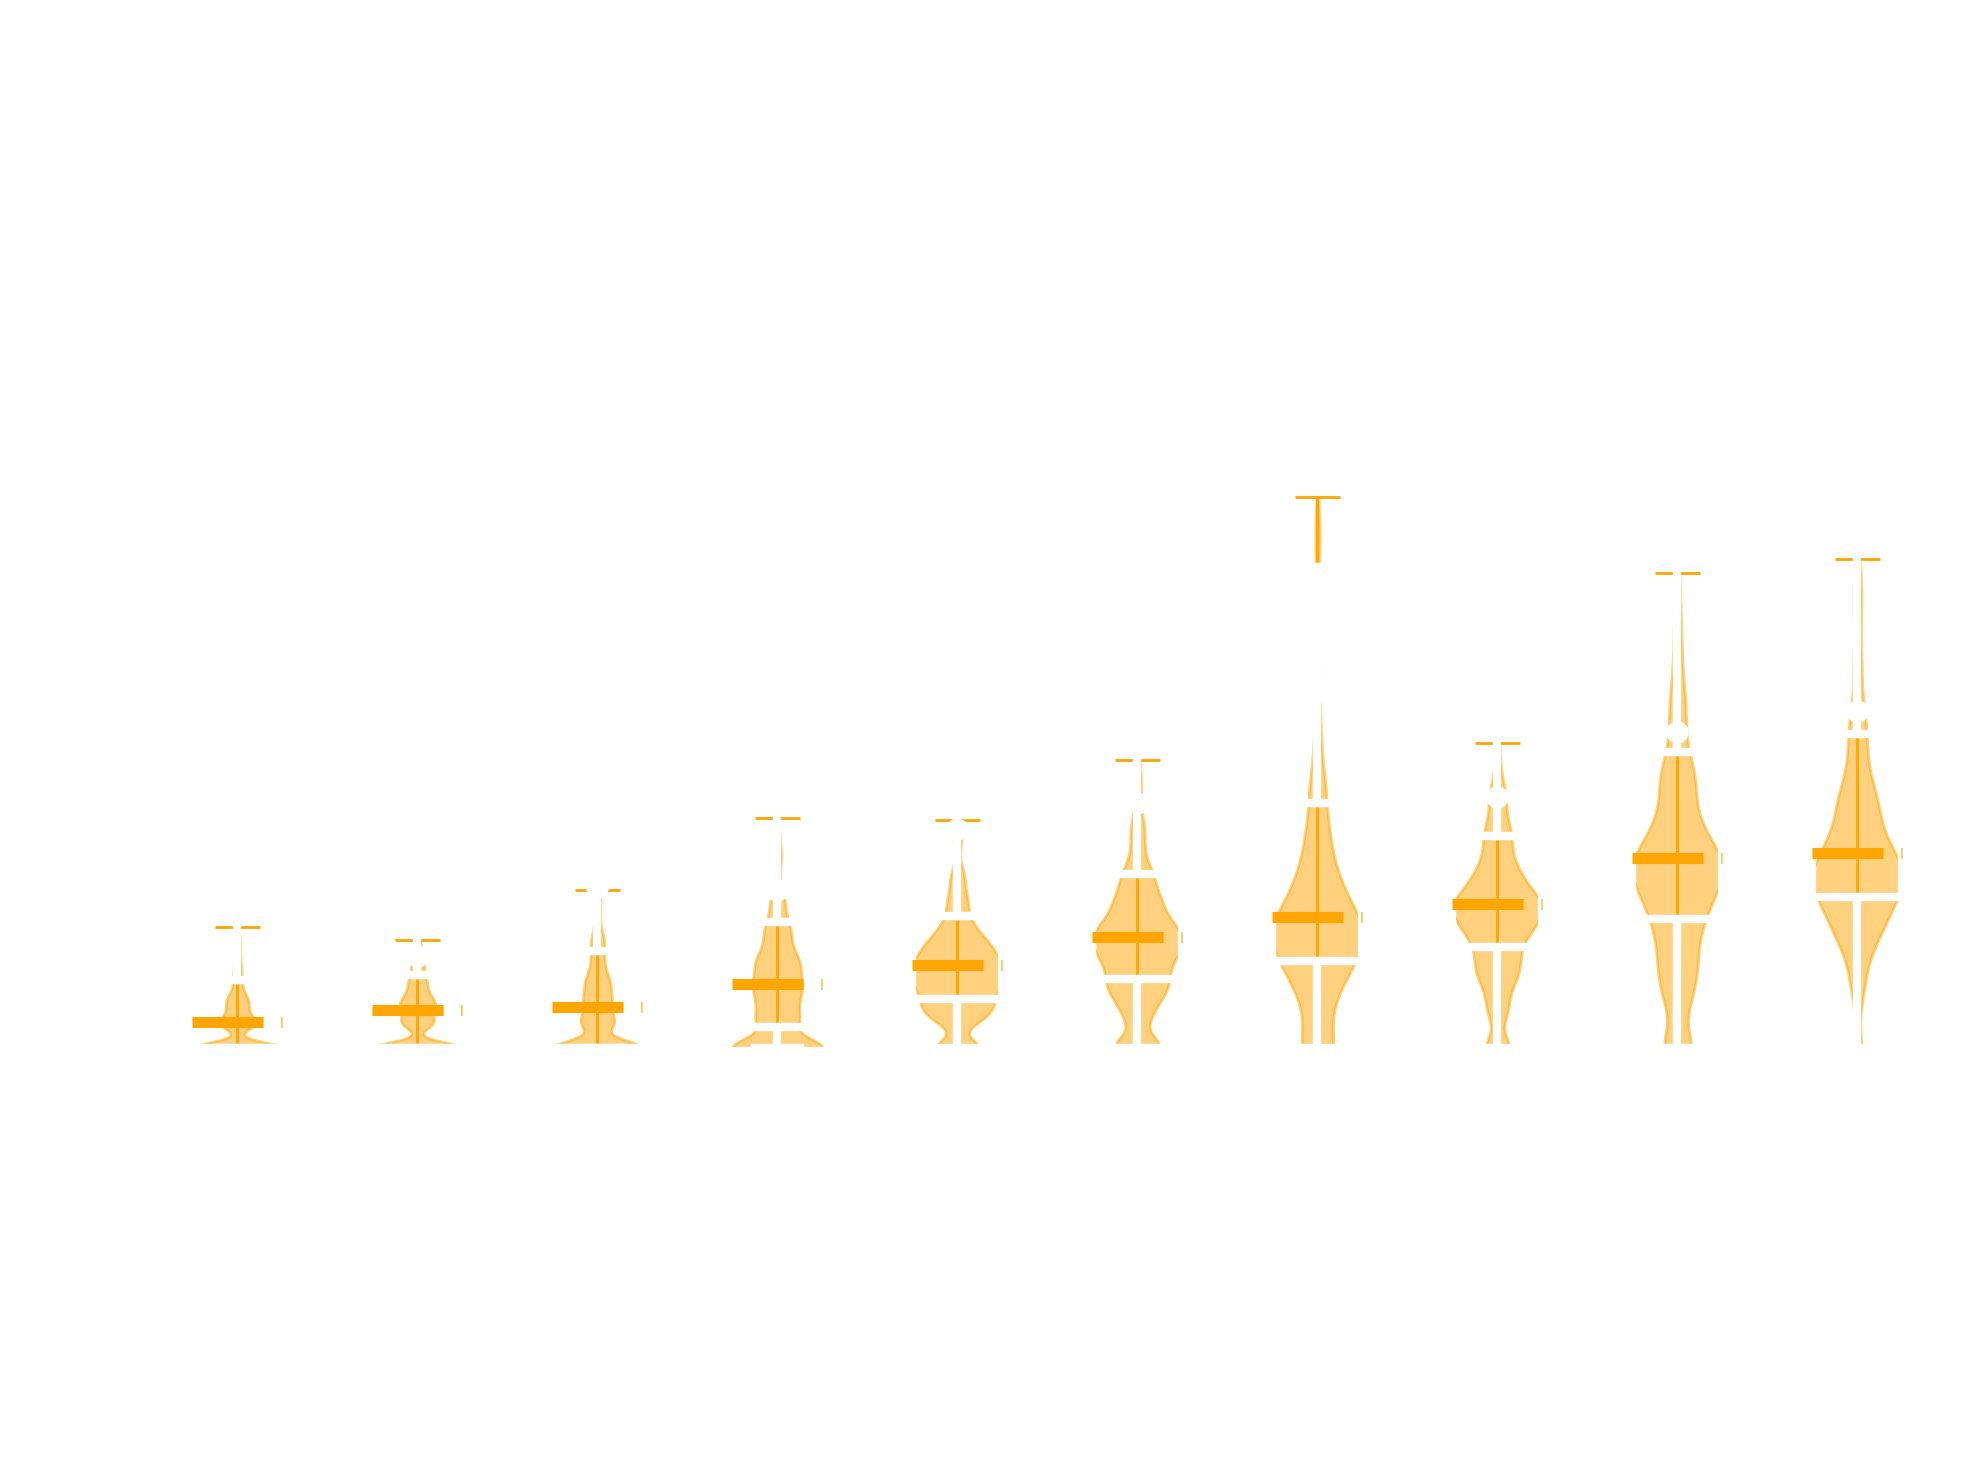
\includegraphics[width=.45\textwidth]{static/performances_standard.png}
        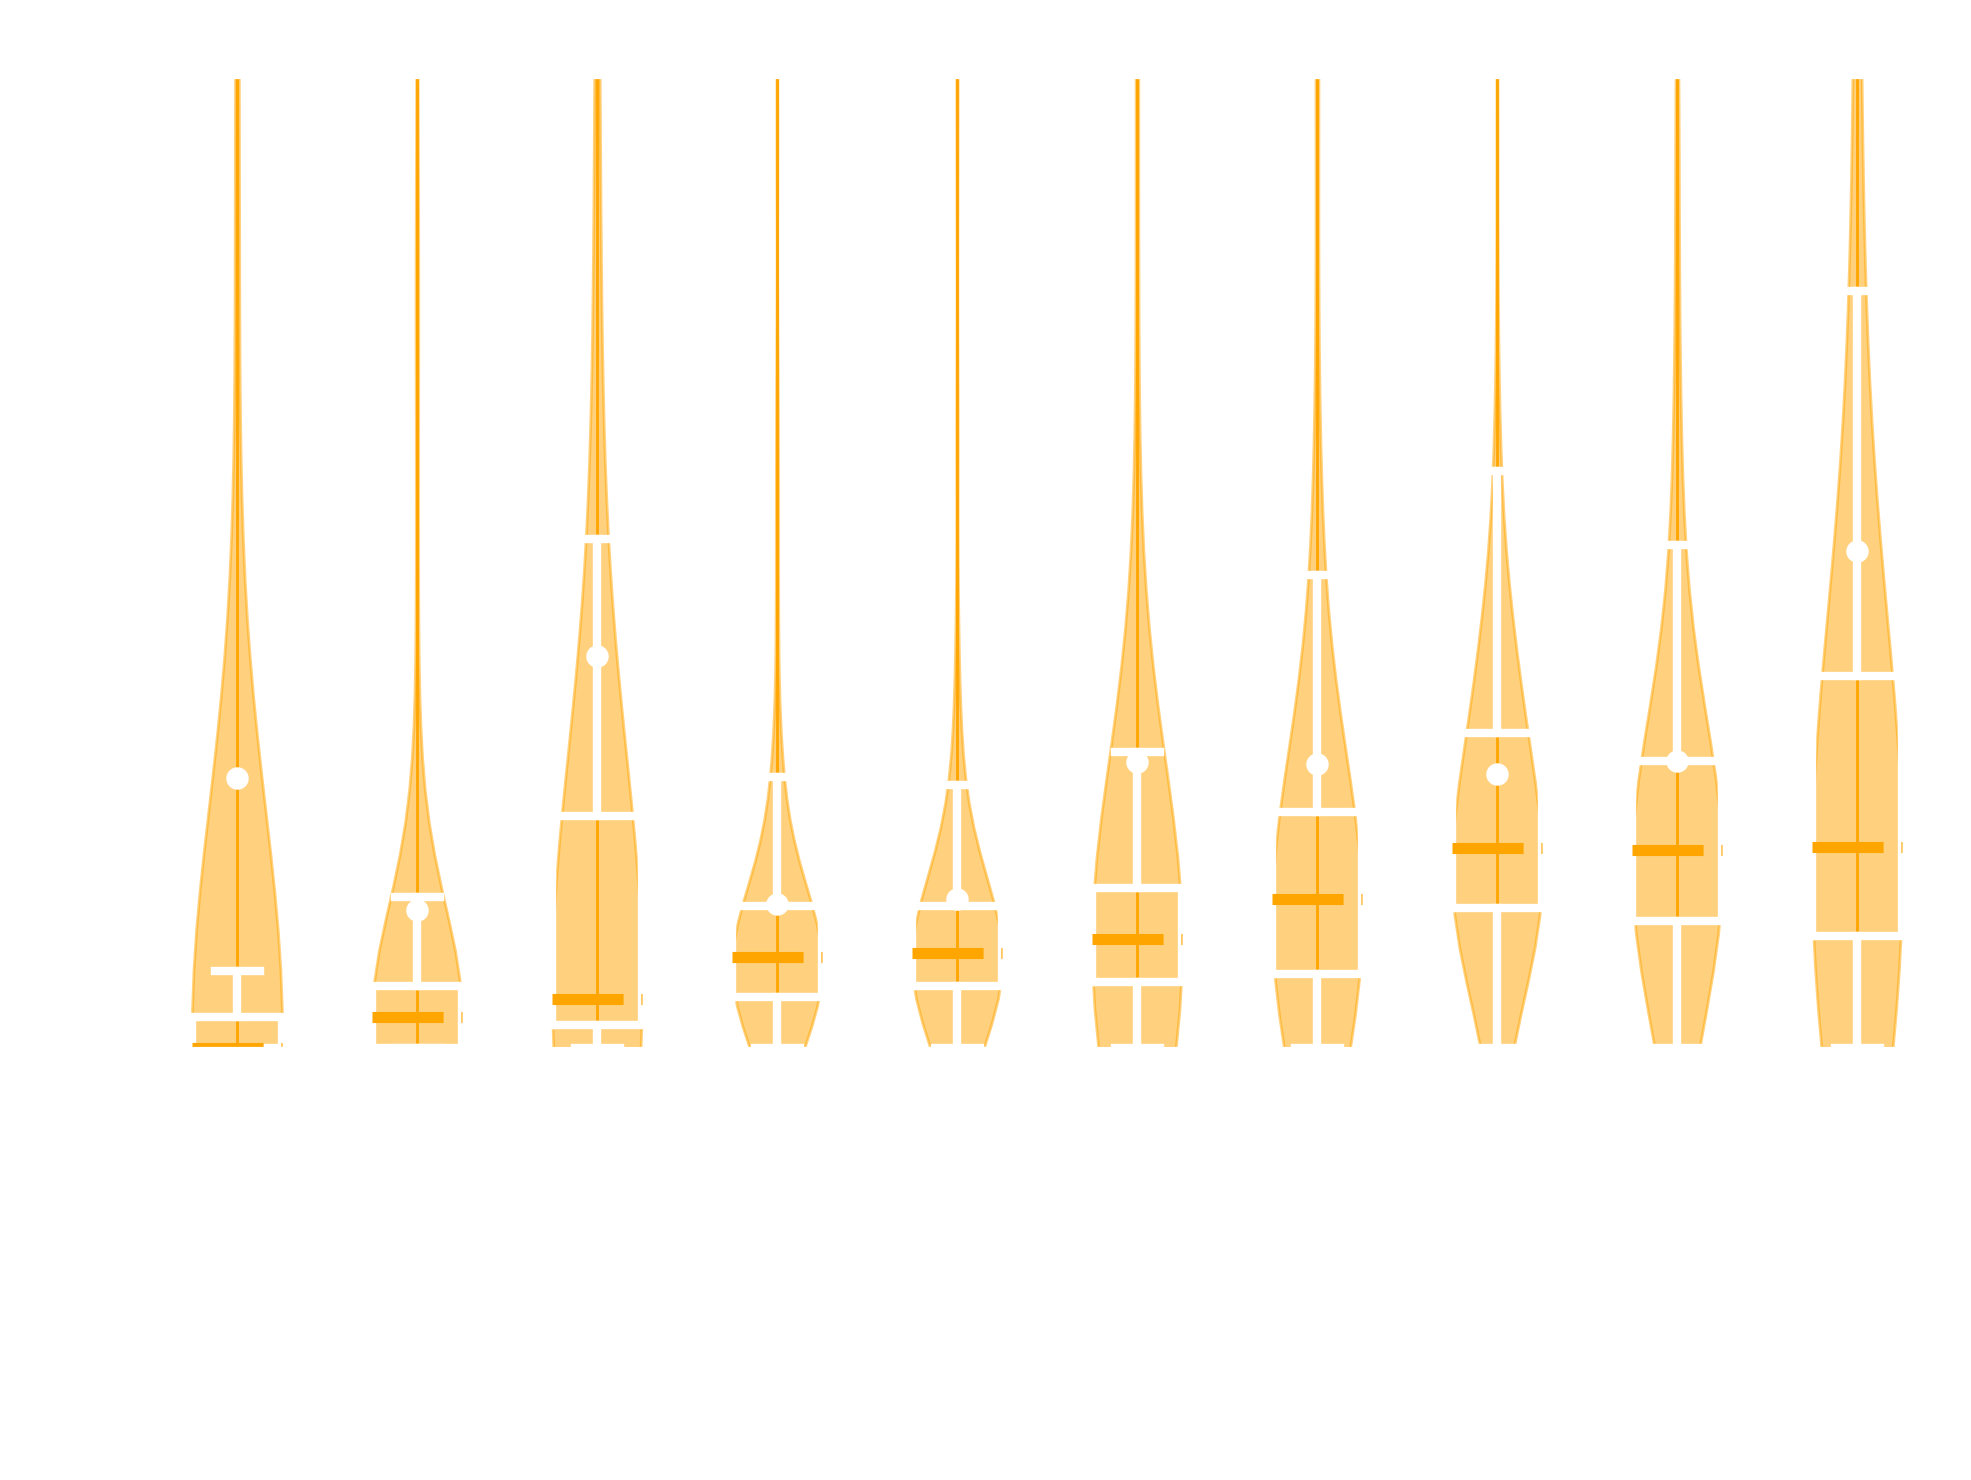
\includegraphics[width=.45\textwidth]{static/performances_noisy.png} \\
        \includegraphics[width=.45\textwidth]{"static/performances_probabilistic ending".png}
        \includegraphics[width=.45\textwidth]{"static/performances_noisy probabilistic ending".png}
    \end{center}
\end{frame}

\begin{frame}
    \begin{center}
        \Large{\textbf{\textcolor{orange}{Highlights \& Challenges}}}
    \end{center}
    \vspace{.8cm} \pause

    \begin{minipage}{.5\textwidth}
    \(\bullet\) Largest collection of strategies  \vspace{.1cm} \\ \pause
    \(\bullet\) Largest number of computer tournaments \vspace{.1cm} \\ \pause
    \(\bullet\) Diverse type of computers tournaments  \vspace{.1cm} \\ \pause
    \(\bullet\) Generalised results \pause
    \end{minipage} \hfill
    \begin{minipage}{.45\textwidth}
    \(\bullet\) Handling big data \vspace{.1cm} \\
    \end{minipage}
\end{frame}

\begin{frame}
    \begin{center}
        \large{``A theory of mind: Best responses to memory-one strategies. The limitations of extortion and restricted memory''} \\ \vspace{.5cm}
        \footnotesize{Nikoleta E. Glynatsi, Vincent A. Knight} \\ \vspace{.5cm}
        \footnotesize{arXiv:1911.12112} \\ \vspace{.5cm}

        \footnotesize{Under review: Scientific Reports}
    \end{center}
\end{frame}

\begin{frame}
    \begin{center}
        \includestandalone[width=.5\textwidth]{static/equations}
    \end{center}
\end{frame}

\begin{frame}
    \begin{center}
        \Large{\textbf{\textcolor{orange}{Highlights \& Challenges}}}
    \end{center}
    \vspace{.8cm} \pause

    \begin{minipage}{.5\textwidth}
        \(\bullet\) New theorem on the utility of a memory-one strategy  \vspace{.1cm} \\ \pause
        \(\bullet\) New mathematical approach for the limitations of memory-one strategies\vspace{.1cm} \\ \pause
        \(\bullet\) Resultant theory \vspace{.1cm} \\ \pause
    \end{minipage} \hfill
    \begin{minipage}{.45\textwidth}
        \(\bullet\) Non convexity of utility function \vspace{.1cm} \\
    \end{minipage}
\end{frame}

\begin{frame}
    \begin{center}
        \large{``Training long short-term memory networks produces successful Prisoner's Dilemma strategies''} \\ \vspace{.5cm}
        \footnotesize{data: DOI:10.5281/zenodo.3685251}
    \end{center}
\end{frame}

\begin{frame}
    \begin{center}
    \includestandalone[width=.9\textwidth]{static/best_sequences_part_two}
    \end{center}
\end{frame}

\begin{frame}
    \begin{center}
    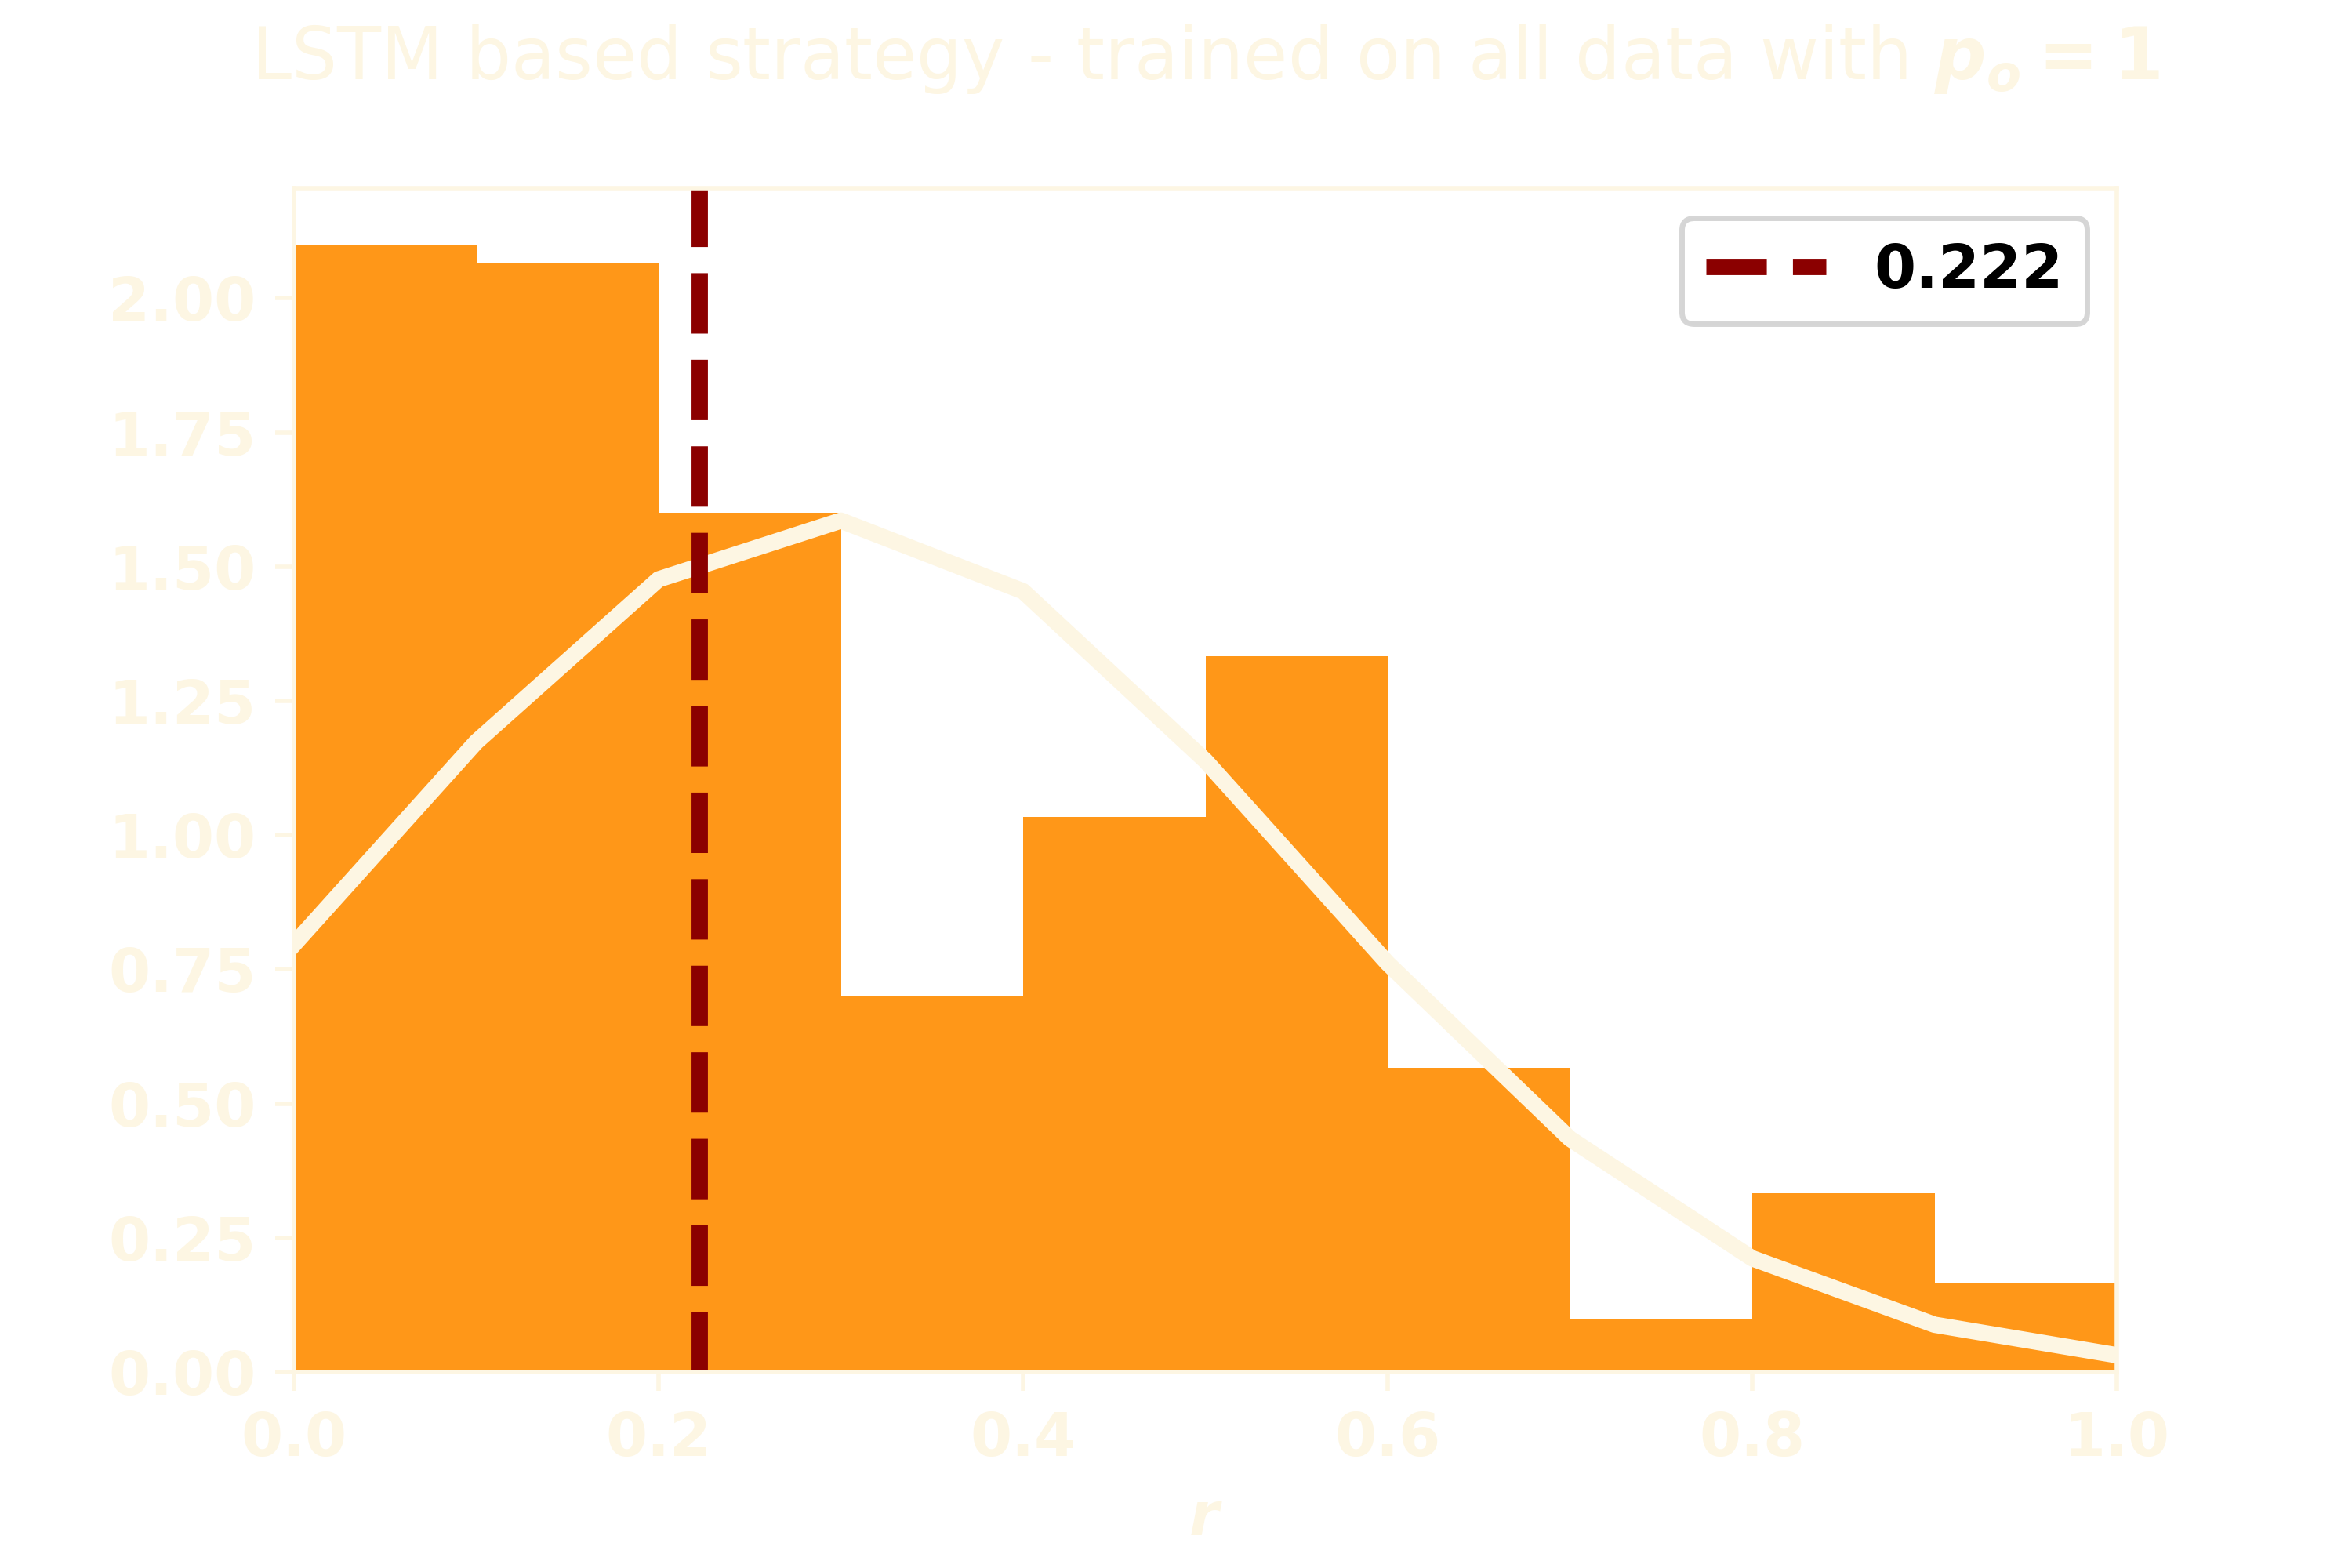
\includegraphics[width=.75\textwidth]{static/lstm_result.png}
    \end{center}
\end{frame}

\begin{frame}
    \begin{center}
        \Large{\textbf{\textcolor{orange}{Highlights \& Challenges}}}
    \end{center}
    \vspace{.8cm} \pause

    \begin{minipage}{.5\textwidth}
        \(\bullet\) Best response sequences using heuristics  \vspace{.1cm} \\ \pause
        \(\bullet\) Artificial neural networks \vspace{.1cm} \\ \pause
        \(\bullet\) Long short-term memory \vspace{.1cm} \\ \pause
        \(\bullet\) Training on GPU \vspace{.1cm} \\ \pause
        \(\bullet\) Promising results of new \\ approach \pause
    \end{minipage} \hfill
    \begin{minipage}{.45\textwidth}
        \(\bullet\) High computational cost \vspace{.1cm}
    \end{minipage}
\end{frame}

\begin{frame}
    \begin{center}
    \large{\textbf{\textcolor{orange}{Be nice \& Open with cooperation}}} \vspace{1cm} \\ \pause
    \large{\textbf{\textcolor{orange}{Be a little envious \& Be complex}}} \vspace{1cm} \\ \pause
    \large{\textbf{\textcolor{orange}{Adapt to the environment \& Longer memory}}}
    \end{center}
\end{frame}

\begin{frame}
    \begin{center}
    \begin{minipage}{.5\textwidth}
        \LARGE{CORRECTNESS}
    \end{minipage}
    \begin{minipage}{.3\textwidth}
        \normalsize{[ko - rektnas]}
    \end{minipage}
    \vspace{.5cm}

    \hspace{-8cm} \normalsize{[noun]}\\
    \end{center}
    \hspace{.8cm} \normalsize{1. the quality or state of being free from error; accuracy.}

\end{frame}


\begin{frame}
    \begin{center}
        \small{\textbf{\textcolor{orange}{Data sets}}} \\
        \scriptsize{\url{doi.org/10.5281/zenodo.3406544}} \\
        \scriptsize{\url{doi.org/10.5281/zenodo.3406542}} \\
        \scriptsize{\url{doi.org/10.5281/zenodo.3406536}} \\
        \scriptsize{\url{doi.org/10.5281/zenodo.3516652}} \\
        \scriptsize{\url{doi.org/10.5281/zenodo.3753498}} \\
        \scriptsize{\url{doi.org/10.5281/zenodo.3402179}} \\
        \scriptsize{\url{doi.org/10.5281/zenodo.3685251}} \\
        \scriptsize{\url{doi.org/10.5281/zenodo.3831431}} \\
        \scriptsize{\url{doi.org/10.5281/zenodo.3841932}} \\
        \vspace{.3cm}

        \small{\textbf{\textcolor{orange}{Software Archive}}} \\
        \scriptsize{\url{doi.org/10.5281/zenodo.1127684}} \\
        \scriptsize{\url{doi.org/10.5281/zenodo.3766344}} \\
        \scriptsize{\url{doi.org/10.5281/zenodo.3533146}} \\
        \scriptsize{\url{doi.org/10.5281/zenodo.3829971}} \\
        \vspace{.3cm}

        \small{\textbf{\textcolor{orange}{Software Development}}} \\
        \scriptsize{\url{github.com/ArcasProject/Arcas}} \\
        \scriptsize{\url{github.com/Nikoleta-v3/meta-analysis-of-prisoners-dilemma-tournaments}} \\
        \scriptsize{\url{github.com/Nikoleta-v3/Memory-size-in-the-prisoners-dilemma}} \\
        \scriptsize{\url{github.com/Nikoleta-v3/Training-IPD-strategies-with-RNN}} \\
    \end{center}
\end{frame}

\begin{frame}
    \footnotesize{\textcolor{orange}{Published}}
    \tiny{
    \begin{enumerate}
    \def\labelenumi{\arabic{enumi}.}
    \item
    Reinforcement learning produces dominant strategies for
    the Iterated Prisoner's Dilemma. Marc Harper, Vincent Knight, Martin
    Jones, Georgios Koutsovoulos, \textbf{Nikoleta E. Glynatsi}, Owen Campbell -
    \href{https://journals.plos.org/plosone/article?id=10.1371/journal.pone.0188046}{PLOS
    One} -
    \href{https://arxiv.org/abs/1707.06307}{Preprint arXiv:1707.06307}
    \item
    An evolutionary game theoretic model of rhino horn
    devaluation. \textbf{Nikoleta E. Glynatsi}, Vincent Knight, Tamsin Lee.
    \href{https://www.sciencedirect.com/science/article/pii/S0304380018303260}{Ecological
    Modelling} -
    \href{https://arxiv.org/abs/1712.07640}{Preprint arXiv:1712.07640}
    \item
    Evolution reinforces cooperation with the emergence of
    self-recognition mechanisms: an empirical study of the Moran process
    for the Iterated Prisoner's dilemma. Vincent Knight, Marc Harper,
    \textbf{Nikoleta E. Glynatsi}, Owen Campbell -
    \href{https://journals.plos.org/plosone/article/comments?id=10.1371/journal.pone.0204981}{PLOS
    ONE} -
    \href{https://arxiv.org/abs/1707.06920}{Preprint arXiv:1707.06920}
    \item
    An open framework for the reproducible study of the
    Iterated prisoner's dilemma. Vincent Knight, Owen Campbell, Marc
    Harper et al -
    \href{https://openresearchsoftware.metajnl.com/articles/10.5334/jors.125/}{Journal
    of Open Research Software}
    \end{enumerate}
    }
    
    \footnotesize{\textcolor{orange}{Under review}}
    \tiny{
    \begin{enumerate} \def\labelenumi{\arabic{enumi}.}
        \item A bibliometric study of research topics, collaboration and influence in the field of the Iterated Prisoner's Dilemma.
        \textbf{Nikoleta E. Glynatsi} and Vincent A. Knight -
        Palgrave Communications - \href{https://arxiv.org/abs/1911.12112}{Preprint arXiv:1911.06128}
        \item Game Theory and Python: An educational tutorial to game
        theory and repeated games using Python \textbf{Nikoleta E. Glynatsi} and Vincent A. Knight -
        Journal of Open Source Education
        \href{https://github.com/Nikoleta-v3/Game-Theory-and-Python}{Nikoleta-v3/Game-Theory-and-Python}
        \item A theory of mind: Best responses to memory-one strategies.
        The limitations of extortion and restricted memory. \textbf{Nikoleta E. Glynatsi} and Vincent A. Knight -
        Scientific Reports -
        \href{https://arxiv.org/abs/1911.12112}{Preprint arXiv:1911.12112}
    \end{enumerate}
    }
    
    \footnotesize{\textcolor{orange}{In preparation}}
    \tiny{
    \begin{enumerate} \def\labelenumi{\arabic{enumi}.}
    \item Properties of Winning Iterated Prisoner's Dilemma Strategies. \textbf{Nikoleta E. Glynatsi}, Vincent A. Knight
    and Marc Harper
    - \href{https://arxiv.org/abs/2001.05911}{Preprint arXiv:2001.05911}
    \item Recognising and evaluating the effectiveness of extortion in
    the Iterated Prisoner's Dilemma. Vincent Knight, Marc Harper, \textbf{Nikoleta E. Glynatsi},
    Jonathan Gillard -
    \href{https://arxiv.org/abs/1904.00973}{Preprint arXiv:1904.00973}
    \end{enumerate}
    }
\end{frame}

\end{document}

